% =====================================================================
%  WORKING NOTES (comments only — these do not appear in the compiled PDF)
%  - Numbers come from paper_outputs.py + estimate_h --sweep
%    (map grid eta {0.5,1.5,2.5,3.5}, Delta {48,96,288}, n_obs=2500, n_mc=40;
%     BTC/ETH 5-minute proxy with 1/5/15-min sweep; SPX = Garman-Klass range proxy).
%  - TODO before submission:
%      upload fig1_bias_curves.png and fig2_map_with_assets.png alongside this file.
%      (Citations checked June 2026. STILL TO CONFIRM before send: ftw2019 vs ftw2022 are
%       DISTINCT works (arXiv preprint vs the Math Finance paper), and contdas2024 exact
%       (title/venue/pages) since the framing rests on it.)
%  - SPX is weak, proxy-confounded corroboration (see Section 4.4).
%  - Citations checked against original sources (June 2026).
%  - Compiles with pdflatex (no .bib needed; references are in thebibliography).
% =====================================================================
\documentclass[11pt]{article}

\usepackage[utf8]{inputenc}
\usepackage[T1]{fontenc}
\usepackage[a4paper,margin=1in]{geometry}
\usepackage{amsmath,amssymb}
\usepackage{booktabs}
\usepackage{graphicx}
% Optional polish on a full TeX Live (e.g. Overleaf): \usepackage{microtype}
\usepackage{xcolor}
\definecolor{linkblue}{rgb}{0.10,0.30,0.55}
\usepackage{hyperref}
\hypersetup{colorlinks=true,allcolors=linkblue}

\setlength{\emergencystretch}{3em}  % absorb rare hard-to-break lines

\title{When is volatility roughness identifiable?\\
A simulation-grounded audit of Hurst estimation from realised variance,
with application to cryptocurrency}

\author{Michael Lumor\thanks{Independent research programme; University of
Salford. ORCID: \href{https://orcid.org/0009-0000-0326-3891}{0009-0000-0326-3891}.
Code and data: \url{https://github.com/Michaellumor/roughvollab}.}}

\date{June 2026}

\begin{document}
\maketitle

\begin{abstract}
The rough-volatility paradigm holds that log-volatility behaves as a fractional
process with Hurst exponent $H \approx 0.1$, an estimate obtained from
realised-volatility (RV) proxies of latent volatility. A parallel literature
argues that this roughness is partly or wholly an artefact of estimating $H$
through a noisy, discretely-sampled proxy. We do not adjudicate \emph{fact versus
artefact}. Instead we ask a prior question: for what region of model and sampling
parameters is $H$ identifiable from RV at all? Using a verified rough-Bergomi
simulator as ground truth---and, crucially, a smooth (semimartingale) null---we
audit the operating characteristics of three roughness estimators (a
structure-function regression, a model-free $p$-variation index, and multifractal
detrended fluctuation analysis) and formalise their behaviour into an
\emph{identifiability map} over the vol-of-vol $\eta$ and the proxy sampling
window $\Delta$. We then pin $\eta$ to data, rather than assuming it, by matching
the model's daily-log-RV variability to each asset's. Applied to BTC and ETH
(Binance, 2019--2025; $n = 2{,}557$ daily observations) and to the S\&P~500
($n = 1{,}759$), the calibration forces $\eta \gtrsim 1.5$, and at that calibrated
$\eta$ no estimator returns an identified reading: the inversion is non-identified,
undefined, or beyond the model's range. The identifiable region is non-empty---%
multifractal DFA recovers roughness across roughly $30\%$ of the grid, concentrated
at fine sampling---but the real assets do not fall in it. This reframes the debate:
the ``rough'' and ``artefact'' readings are two answers to a single ill-posed
inverse problem. All code, data tooling, and figures are open and reproducible.

\medskip
\noindent\textbf{Keywords:} rough volatility, Hurst exponent, realised variance,
identifiability, fractional Brownian motion, cryptocurrency.
\end{abstract}

% =====================================================================
\section{Introduction}

Since Gatheral, Jaisson and Rosenbaum's observation that log-volatility scales
like a fractional Brownian motion with a small Hurst exponent (GJR 2018),
``rough volatility'' has become a major modelling paradigm: the rough-Bergomi and
rough-Heston models reproduce features of the implied-volatility surface that
classical models miss. The empirical claim $H \approx 0.1$ rests on estimating the
regularity of a \emph{latent} object---spot volatility---through a \emph{proxy},
typically realised variance computed from high-frequency returns.

That dependence on a proxy is the source of an ongoing dispute. Cont and Das
(2024) show, with a model-free $p$-variation estimator, that the roughness measured
from realised-volatility signals can arise from the proxy and microstructure noise
rather than from the latent volatility itself, and they question whether the
evidence supports genuinely rough sample paths. Rogers (2023) raises related
concerns about over-interpreting the estimate. A countervailing literature defends
the finding with more careful estimators: Fukasawa, Takabatake and Westphal
(``Is volatility rough?'') and Bolko, Christensen, Pakkanen and Veliyev (2023)
propose quasi-likelihood and GMM procedures, respectively, and Bennedsen, Lunde and
Pakkanen (2022) study the short- and long-memory structure directly. The
literature, in short, divides into \emph{fact} and \emph{artefact}.

We argue that this framing skips a prior question. Before asking whether volatility
\emph{is} rough, one should ask whether $H$ is identifiable from a realised-variance
proxy at all, and under what conditions. Estimation error and observational
equivalence are properties of an inverse problem---recovering a latent parameter
through a noisy, discretely-sampled, aggregated proxy---and the answer depends on
the vol-of-vol and on how finely the proxy is sampled. Our contribution is to make
that dependence explicit, to calibrate the one free knob ($\eta$) to data rather
than assume it, and to locate real assets on the resulting map.

\medskip
\noindent\textbf{Contributions.}
\begin{enumerate}
\item \textbf{A simulation-grounded audit} of three roughness estimators against a
verified rough-Bergomi generator \emph{and a smooth null}, characterising each
estimator's finite-sample bias as a function of true $H$, $\eta$ and $\Delta$. The
smooth null is essential: without it, an audit cannot detect spurious roughness.
\item \textbf{An operational definition of identifiability} for the RV inverse
problem, and an \textbf{identifiability map} that classifies each $(\eta, \Delta)$
regime as \emph{identified}, \emph{de-biasable}, or \emph{non-identified} per
estimator. The map shows that an identifiable region exists but is restricted,
contracting at coarse sampling and depending sharply on $\eta$.
\item \textbf{A data calibration of $\eta$} that closes the ``just assume small
vol-of-vol'' escape hatch: matching the model's daily-log-RV variability to an
asset's forces $\eta \gtrsim 1.5$ for cryptocurrency, and at that $\eta$ the
roughness reading is non-identified.
\item \textbf{Cross-asset empirical placement}: BTC, ETH and the S\&P~500 fall
\emph{outside} the identifiable region. We read this not as ``volatility is smooth''
but as ``the roughness of these assets is not identified from this proxy at their
calibrated vol-of-vol.''
\item \textbf{Full reproducibility}: an open repository with a verified simulator, a
stdlib-only data pipeline, a test suite, and one-command figure regeneration.
\end{enumerate}

The work is undergraduate-led and deliberately scoped: it audits operating
characteristics by simulation rather than proving identifiability theorems, and it
is offered as a careful, open, reproducible contribution to a contested empirical
question.

% =====================================================================
\section{Related work}

\noindent\textbf{The rough paradigm.} Fractional Brownian motion (Mandelbrot and
Van Ness 1968) underlies rough volatility; GJR (2018) gave the empirical case, and
Bayer, Friz and Gatheral (2016) the pricing model; the edited volume of Bayer,
Friz, Fukasawa, Gatheral, Jacquier and Rosenbaum (2024) collects the modelling and
asymptotic results.

\medskip
\noindent\textbf{Estimation and its critique.} Estimating $H$ from discrete data
was studied by Rosenbaum and co-authors well before the volatility application. In
the volatility setting, Cont and Das (2024) introduce a normalised $p$-variation
roughness index and identify a proxy-error mechanism by which realised-volatility
signals appear rougher than the latent process; Cont and Das (2023) develop the
underlying pathwise theory. Fukasawa, Takabatake and Westphal (``Is volatility
rough?'') and Bolko et al.\ (2023) defend the rough estimate with likelihood- and
moment-based methods that attempt to correct for the proxy. Bennedsen, Lunde and
Pakkanen (2022) decouple short- and long-term behaviour. For cryptocurrency
specifically, Takaishi (2020) reports rough-volatility and multifractality results
for Bitcoin.

\medskip
\noindent\textbf{Realised variance and microstructure.} Realised variance as a
volatility proxy is standard (Andersen, Bollerslev, Diebold and Labys 2003);
bipower variation provides jump robustness (Barndorff-Nielsen and Shephard 2004).
For equities without intraday data we use the Garman--Klass (1980) range estimator.
Microstructure noise biases RV at the finest sampling frequencies, a key confound
for any roughness measurement.

Our position relative to this body of work is orthogonal to the fact/artefact axis:
we characterise the identifiability of the inverse problem itself, and locate assets
on that characterisation.

% =====================================================================
\section{Methods}

\subsection{Estimators}

We audit three estimators of the roughness of a one-dimensional log-volatility
series, chosen because they rest on different principles and, importantly,
\textbf{disagree in the sign of their small-$H$ bias}:
\begin{itemize}
\item \textbf{GJR structure-function regression.} The $q$th-order structure
function $m(q, \Delta) = \mathbb{E}\,|\log \sigma_{t+\Delta} - \log \sigma_t|^q$ is
regressed on $\log \Delta$ across $q \in \{0.5, 1, 1.5, 2, 3\}$; $H$ is read from
the slope divided by $q$, with monofractality checked via the linearity of the
scaling exponent in $q$. Empirically this estimator biases \emph{upward} at small
true $H$.
\item \textbf{Cont--Das normalised $p$-variation index.} A model-free roughness
index based on normalised $p$-th variation along a sequence of partitions. It also
biases \emph{upward} at small $H$ and, on real data, frequently returns no finite
estimate.
\item \textbf{MF-DFA.} The generalised Hurst exponent from multifractal detrended
fluctuation analysis ($H = h(2) - 1$), which doubles as a multifractality
diagnostic. It biases \emph{downward} at small $H$.
\end{itemize}

The sign-disagreement is not a nuisance to be averaged away; it is diagnostic. When
three principled estimators err in opposite directions, their disagreement is itself
information about how ill-posed the underlying inversion is.

\subsection{Ground-truth generators}

The audit requires a ground truth whose roughness is known. We use a verified
$\kappa = 0$ Volterra engine to generate rough log-variance paths under the RFSV /
rough-Bergomi specification,
\[
  \log V_t = \log \xi_0 + \eta\, \widetilde{W}_t - \tfrac{1}{2}\,\eta^2 v_t,
\]
where $\widetilde{W}$ is the rough (Volterra) process of Hurst exponent $H$ and
$v_t$ its variance function; by construction $\mathbb{E}[V_t] = \xi_0$ and
$\log V_t$ inherits Hurst exponent $H$. We sweep
$H \in \{0.05, 0.10, 0.15, 0.20, 0.30, 0.45\}$ and, crucially, include a
\textbf{smooth null}: a Markovian log-Ornstein--Uhlenbeck volatility with effective
$H = 1/2$. An audit that cannot distinguish a genuinely rough process from a smooth
one \emph{that has been passed through the same proxy} cannot certify any roughness
measurement.

\subsection{The realised-variance proxy and corruption ladder}

Estimators consume not the latent log-variance but a realised-variance proxy:
returns are squared and summed within calendar bars to form a daily log-RV series,
the same object built from real data. To separate genuine roughness from proxy
artefacts we apply a \emph{corruption ladder}---a sequence of controlled distortions
to a rough ground truth---and measure each estimator's response: (i) the RV-proxy
bias envelope; (ii) microstructure noise and subsampling; (iii) jumps, with a
bipower-variation robust twin; (iv) finite-sample effects; and (v)
calendar/day-of-week seasonality, which we show biases the estimators in opposite
directions and is fully removed by deseasonalising. The ladder establishes which
distortions are removable and which are not.

\subsection{An operational definition of identifiability}
\label{sec:iddef}

The audit yields, for each measurement configuration $(\eta, \Delta, \text{series
length})$, a \emph{bias curve}: the map from true $H$ to the expected observed
estimate $\mathbb{E}[\hat H]$, with a single-sample spread $\sigma$ obtained by
Monte Carlo over independent paths of the same length as the data. Identifiability
is a property of this curve. We call a true $H$, under a given estimator and
configuration:
\begin{itemize}
\item \textbf{non-identified} if the bias curve is non-monotone over the $H$
grid---then a rough and a much smoother true $H$ yield the \emph{same} observed
estimate (observational equivalence), so the inversion is multivalued---or if its
local slope falls below a floor, so that many true $H$ map to nearly the same
observed estimate (the collapse);
\item \textbf{identified} if the curve is monotone and well-posed \emph{and} the
$\pm z\sigma$ single-sample band around the observed estimate inverts to an
implied-true-$H$ interval lying entirely below $H = 1/2$---so the data could
conclude ``rough'' with confidence by excluding the smooth null;
\item \textbf{de-biasable} if the inversion is unique but the band cannot exclude
the smooth null (point-estimable, but rough and smooth are not separable at the
available precision).
\end{itemize}

This definition is applied identically to simulated configurations and to real
data, so a real asset's status is computed by exactly the rule used to draw the map.

\subsection{Calibrating the vol-of-vol to data}

The identifiable region depends on $\eta$, and $\eta$ is not directly observed.
Rather than assume a value, we pin it per asset: the vol-of-vol controls the
dispersion of daily log-RV, so we choose $\eta$ so that the model's daily-log-RV
standard deviation matches the asset's own. This quantity is monotone in $\eta$, so
the calibration is a one-dimensional root-find; when an asset is more variable than
the model produces at any $\eta$ in the search range, $\eta$ is clamped at the
boundary---the honest ``the model is calmer than the asset at every $\eta$ we
tried'' outcome.

\subsection{The identifiability map}

Sweeping the bias-curve construction over a grid of $(\eta, \Delta)$ and classifying
every cell yields the identifiability map: for each estimator, a panel per $\Delta$
with $\eta$ on one axis and true $H$ on the other, each cell coloured by status. An
asset is placed on the panel matching its proxy window, at its calibrated $\eta$, at
the implied true $H$ obtained by inverting its observed estimate against the matched
curve; below-floor and multivalued assets are drawn as off-grid and bracketed
markers, respectively, rather than as a fictitious point.

% =====================================================================
\section{Results}

\subsection{Estimator operating characteristics}

The audit reproduces the expected sign-disagreement: GJR and Cont--Das over-estimate
roughness at small true $H$ while MF-DFA under-estimates it (Figure~\ref{fig:bias}).
On the corruption ladder, the RV proxy alone is sufficient to manufacture apparent
roughness from a smooth null; microstructure noise and finite-sample effects deepen
the bias; calendar seasonality biases the estimators in opposite directions and is
exactly recoverable by deseasonalising. These results establish that a na\"ive
roughness reading from RV cannot be trusted without the audit, and that some---but
not all---distortions are removable.

\begin{figure}[t]
\centering
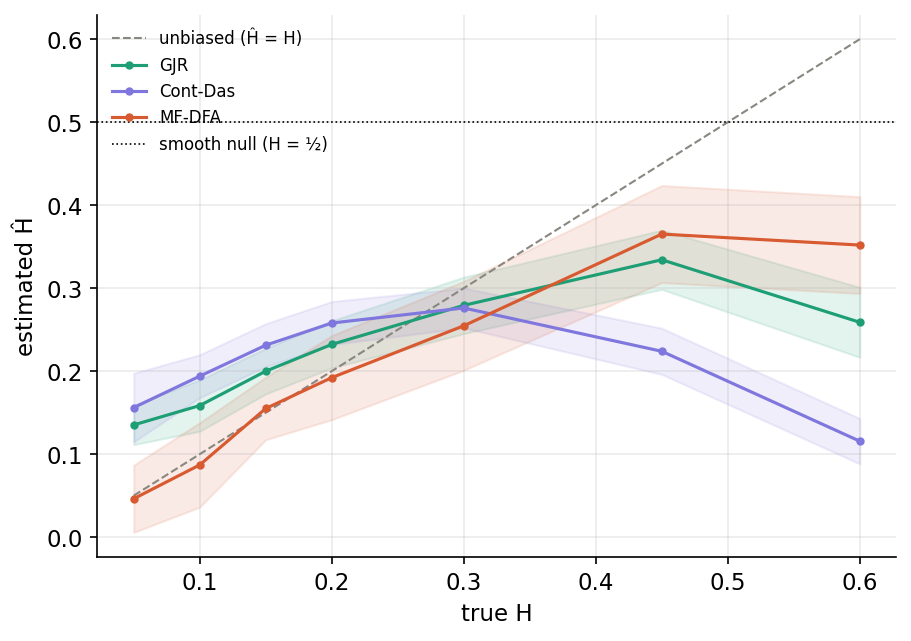
\includegraphics[width=0.78\textwidth]{fig1_bias_curves.png}
\caption{Estimator bias curves: $\mathbb{E}[\hat H]$ versus true $H$ for GJR,
Cont--Das and MF-DFA at $\eta = 1.5$, $\Delta = 288$, with the smooth-null reference
(dotted, $H = \tfrac{1}{2}$) and the unbiased diagonal. GJR and Cont--Das
over-estimate roughness at small $H$ while MF-DFA sits lower, and the estimators
diverge sharply at large $H$ --- the sign disagreement that makes the inversion
ill-posed.}
\label{fig:bias}
\end{figure}

\subsection{The identifiability map}

The map (Figure~\ref{fig:map}) shows that \textbf{an identifiable region exists but
is restricted and concentrated at fine sampling}. Across the $(\eta, \Delta, H)$
grid---$\eta \in \{0.5, 1.5, 2.5, 3.5\}$, $\Delta \in \{48, 96, 288\}$ bars---%
multifractal DFA recovers roughness in about $30\%$ of cells and the
structure-function (GJR) estimator in about $12\%$, with the identified cells
clustered at the finest window ($\Delta = 288$) and all but vanishing at coarse
sampling. The model-free Cont--Das index is identifiable almost nowhere (about
$92\%$ non-identified) and returns no finite estimate over a further $8\%$. The
identifiable region contracts sharply at coarser sampling and shifts with $\eta$,
consistent with the proxy-error mechanism intensifying as vol-of-vol grows.

The headline of this figure is \emph{not} ``nothing is identifiable.'' It is that
the method works in principle across a real region of parameter space---which makes
the subsequent empirical finding much harder to dismiss as an artefact of weak
estimators.

\begin{figure}[t]
\centering
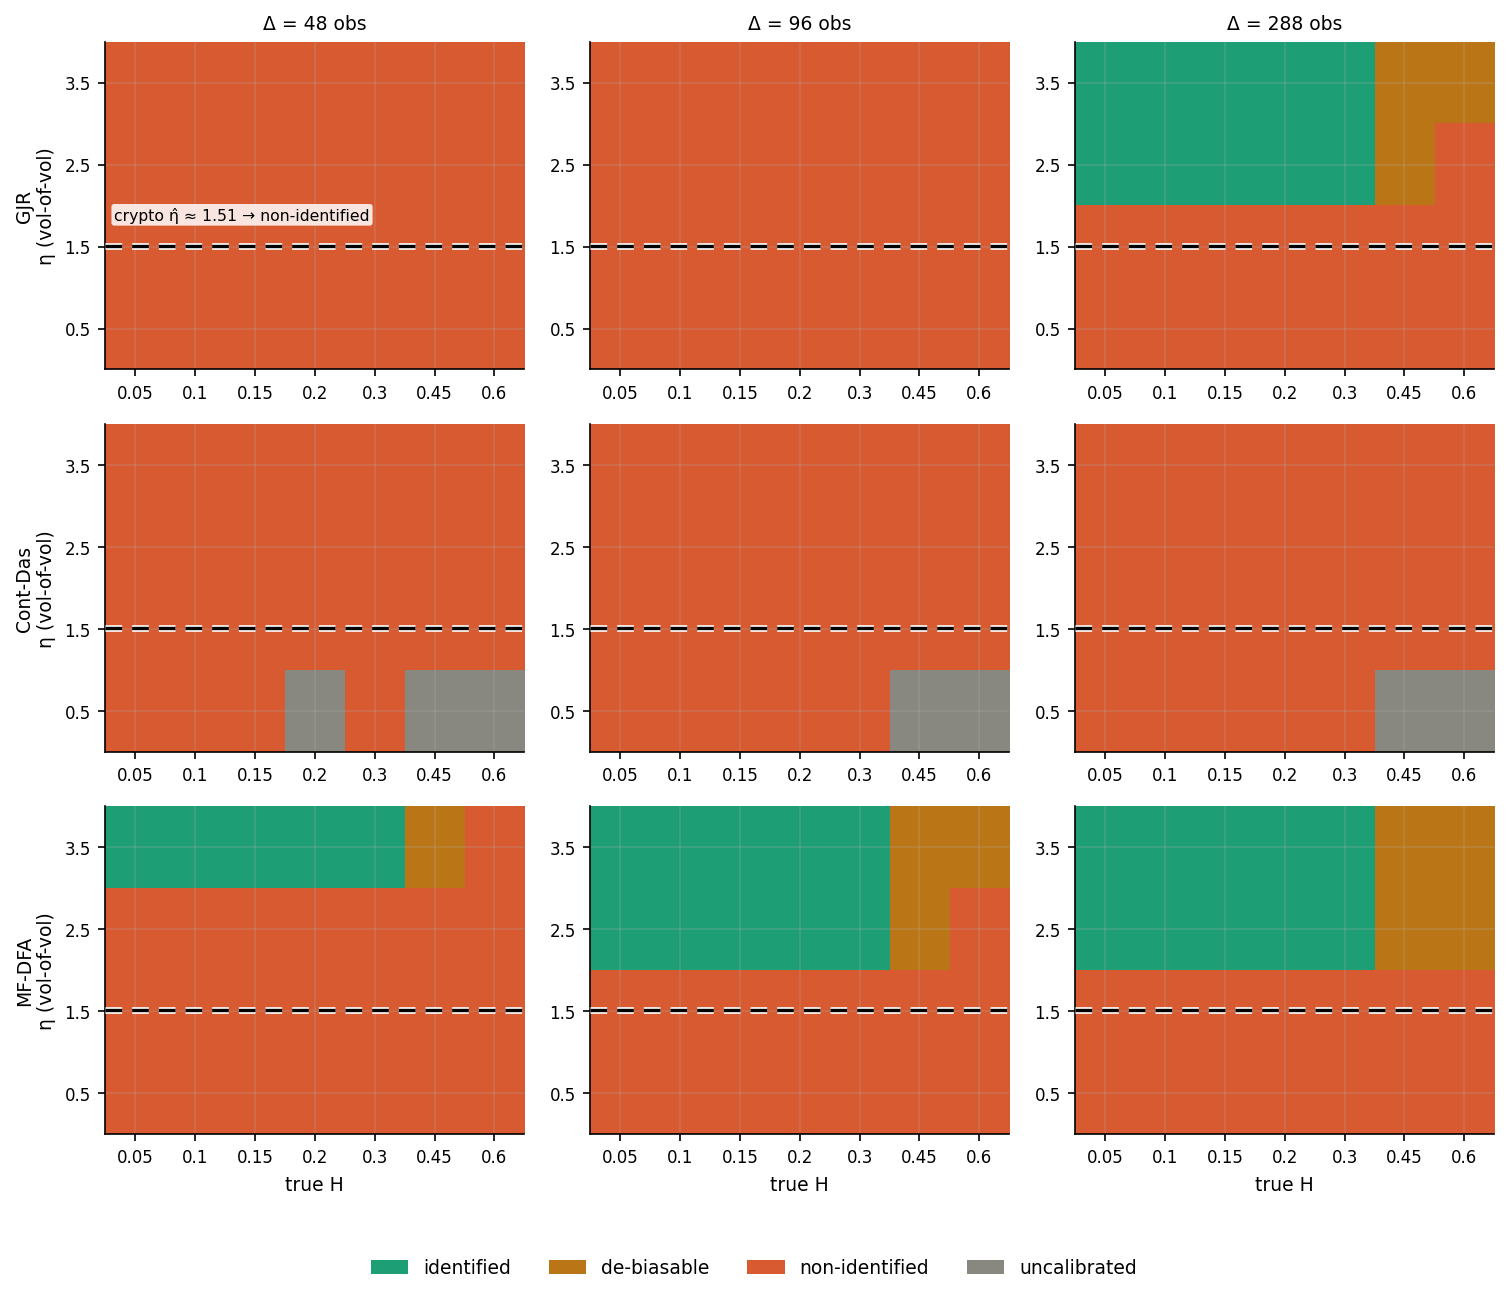
\includegraphics[width=\textwidth]{fig2_map_with_assets.png}
\caption{The identifiability map: estimators in rows, sampling window $\Delta \in
\{48, 96, 288\}$ in columns, each panel with $\eta \times$ true-$H$ cells coloured
identified / de-biasable / non-identified. The dashed line marks crypto's
calibrated vol-of-vol ($\hat\eta \approx 1.5$; BTC $1.57$, ETH $1.45$), which lies
in the non-identified band on every estimator and at every sampling window.}
\label{fig:map}
\end{figure}

\subsection{Locating real assets}
\label{sec:assets}

We compute daily log-RV for BTC and ETH from Binance 1-minute klines (2019--2025;
$n = 2{,}557$ daily observations), sampled at 5 minutes ($\Delta = 288$ returns per
bar). The structure-function estimator reads $\hat H = 0.083$ for BTC and
$\hat H = 0.070$ for ETH, with clean monofractal scaling ($R^2 = 0.99$). Crucially,
these readings are stable across sampling frequency and do \emph{not} fall as
sampling becomes finer---the opposite of the microstructure-noise signature, which
rules that confound out (Table~\ref{tab:sweep}).

\begin{table}[t]
\centering
\caption{Sampling sweep: $\hat H$ versus RV sampling window. The structure-function
($\hat H_{\mathrm{GJR}}$) estimate is flat (or rising) as sampling becomes finer,
the opposite of the microstructure-noise signature.}
\label{tab:sweep}
\begin{tabular}{llrrr}
\toprule
Sampling & $n$ & GJR & Cont--Das & MF-DFA \\
\midrule
BTC, 1 min  & $2{,}557$ & $+0.092$ & NaN & $-0.052$ \\
BTC, 5 min  & $2{,}557$ & $+0.083$ & NaN & $-0.057$ \\
BTC, 15 min & $2{,}557$ & $+0.083$ & NaN & $-0.062$ \\
ETH, 1 min  & $2{,}557$ & $+0.077$ & NaN & $-0.056$ \\
ETH, 5 min  & $2{,}557$ & $+0.070$ & NaN & $-0.065$ \\
ETH, 15 min & $2{,}557$ & $+0.070$ & NaN & $-0.076$ \\
\bottomrule
\end{tabular}
\end{table}

The structure-function estimate is flat from 15-minute to 5-minute sampling and
ticks slightly \emph{up} at 1 minute for both assets; were the apparent roughness a
microstructure artefact, $\hat H$ would fall towards $\tfrac{1}{2}$ as the sampling
interval shrank. Cont--Das returns no finite estimate at any frequency, and MF-DFA
is negative throughout---outside the admissible range $[0, 1]$---growing more
negative at coarser sampling. (The multifractality diagnostic is mixed: BTC is
monofractal, $\Delta h(q) \approx 0.04$, while ETH shows a multifractal spread,
$\Delta h(q) \approx 0.08$---a caveat for the monofractal rough-Bergomi ground
truth. We note that our monofractal reading for BTC sits alongside a literature
that has argued the opposite (Takaishi 2025); we record this disagreement rather
than resolve it, and return to it in Section~\ref{sec:limitations}.)

Calibrating $\eta$ to each asset's daily-log-RV variability forces
\textbf{$\hat\eta = 1.57$ for BTC and $\hat\eta = 1.45$ for ETH}, both essentially
at the threshold below which the model cannot reproduce crypto's RV dispersion. At
these calibrated $\eta$, the assets land \textbf{outside the identifiable region on
every estimator} (Figure~\ref{fig:map}, markers):

\begin{table}[t]
\centering
\setlength{\tabcolsep}{4pt}
\caption{Per-asset placement at the calibrated $\hat\eta$. No estimator returns an
\emph{identified} status for either coin.}
\label{tab:assets}
\begin{tabular}{lrrlll}
\toprule
Asset & $n$ & $\hat\eta$ & GJR ($\hat H \to$ status) & Cont--Das & MF-DFA ($\hat H \to$ status) \\
\midrule
BTC & $2{,}557$ & $1.57$ & $0.083 \to$ non-identified & NaN $\to$ uncalibrated & $-0.057 \to$ below-floor \\
ETH & $2{,}557$ & $1.45$ & $0.070 \to$ non-identified & NaN $\to$ uncalibrated & $-0.065 \to$ non-identified \\
\bottomrule
\end{tabular}
\end{table}

No estimator returns an \emph{identified} status for either coin. The
structure-function inversion is non-identified (at the calibrated $\eta$ the bias
curve does not separate the reading from the smooth null); Cont--Das returns no
finite estimate; and MF-DFA produces a \emph{negative} exponent
($\hat H \approx -0.06$), physically impossible and below the model's floor. Three
principled methods fail in three different ways---non-identified, undefined, out of
range---all pointing to the same conclusion: the roughness of these assets is not
identified from this proxy at their data-implied vol-of-vol.

\subsection{Equity corroboration}
\label{sec:equity}

For the S\&P~500 we form a Garman--Klass range proxy from daily OHLC ($n = 1{,}759$),
the range proxy being trading-session-only (no overnight gap). The structure-function
reading, $\hat H = 0.132$, is \emph{less} rough than crypto---the direction expected
from the calendar/gap difference. We report the equity result only as \textbf{weak
corroboration}, because it is confounded by the proxy. The range proxy's
daily-log-variance is far less dispersed than an intraday-RV sum, so the vol-of-vol
calibration bottoms out at the search floor ($\hat\eta = 0.20$, clamped); at that
$\eta$ the structure-function and MF-DFA readings both fall \emph{above} the model's
range (above-ceiling) and Cont--Das is undefined. As with crypto, then, no estimator
returns an identified status---but here the non-identification is entangled with a
range-versus-RV proxy mismatch rather than cleanly established. A proper equity test
needs intraday returns to build a comparable RV proxy; the clean isolation of the
calendar effect remains the controlled simulation in the corruption ladder, not this
comparison.

% =====================================================================
\section{Discussion}

\subsection{Reframing fact versus artefact}

The fact and artefact positions are, on this account, two readings of a single
ill-posed inverse problem. The map makes the structure explicit: there is a region
of $(\eta, \Delta)$ where roughness is recoverable, and the disputed quantity for
real assets sits \emph{outside} it once $\eta$ is fixed to data. One need not decide
whether volatility ``is'' rough to observe that, for these assets at this proxy and
this vol-of-vol, the question is not answerable from the data---the rough and smooth
hypotheses are observationally equivalent through the proxy.

\subsection{Why this is stronger than a null result}

A blanket ``you cannot measure $H$'' claim is easy to dismiss as a weak-estimator
artefact. The identifiability map forecloses that response: the same estimators, on
simulated data, \emph{do} recover roughness across a real region of parameter space.
The finding is the juxtaposition---identifiable region present, assets outside
it---not the absence of identifiability everywhere.

\subsection{Limitations}
\label{sec:limitations}

Several caveats bound the claim, and should bound how the result is read.
\begin{itemize}
\item \textbf{Model-relative calibration.} $\hat\eta$ is the vol-of-vol that makes
the rough-Bergomi model match an asset's RV variability; it is not a model-free
property of the asset. The non-identification is established relative to this model
class.
\item \textbf{Single model class.} Ground truth is rough-Bergomi with a
$\kappa = 0$ Volterra engine; results may differ under other rough or multifractal
specifications. Bitcoin RV has been argued to be multifractal rather than
monofractal (Takaishi 2025), which our MF-DFA diagnostic can detect---and indeed
flags for ETH---but which we do not model as ground truth.
\item \textbf{Simulation-based, not a theorem.} Identifiability here is
operational---read off finite-sample operating characteristics---not a formal proof
of (non-)identifiability. A likelihood- or GMM-based treatment yielding identified
sets (in the spirit of Fukasawa--Takabatake--Westphal and Bolko et al.) would harden
the inference; we regard this as the natural next step.
\item \textbf{Equity proxy mismatch.} The range proxy is trading-session-only and
not directly comparable to the intraday-RV proxy used for crypto, so the cross-asset
comparison is suggestive, not clean.
\end{itemize}

\subsection{Practical implications}

For calibration and hedging, the practical reading is conservative: a point estimate
of $H$ from realised variance should not be over-trusted for assets whose calibrated
vol-of-vol places them in the non-identified region. Where the roughness parameter
is not identified, decisions that are sensitive to it (for instance, the choice
between a rough and a classical volatility model) cannot be resolved by the RV
evidence alone and should be made robust to the ambiguity.

% =====================================================================
\section{Conclusion}

We have asked, before \emph{is volatility rough?}, the prior question \emph{is its
roughness identifiable from realised variance, and when?} A simulation-grounded
audit against rough and smooth ground truth, formalised into an identifiability map
and combined with a data calibration of the vol-of-vol, shows that an identifiable
region exists but that BTC and ETH fall outside it---at their calibrated $\eta$ the
roughness reading is non-identified, undefined, or out of range across three
principled estimators---with the S\&P~500 yielding no identified reading either,
though confounded by its range proxy. The fact and artefact positions are reconciled
as two readings of one ill-posed inverse problem. The natural next step is to replace
operational identifiability with formal identified sets via a likelihood- or
moment-based estimator, and to test the result across more assets, sampling windows,
and model classes.

% =====================================================================
\section*{Reproducibility statement}

All code, the data-processing pipeline, the test suite, and the figure-generation
scripts are available at \url{https://github.com/Michaellumor/roughvollab}
(ORCID 0009-0000-0326-3891). The simulator is unit-tested against analytic limits;
the data tooling is stdlib-only; every figure regenerates from one command with
documented random seeds. Raw exchange data are downloaded and SHA-verified by the
pipeline rather than redistributed.

% =====================================================================
\section*{Use of generative AI}

The author used a large language model (Anthropic's Claude) extensively as a
research assistant throughout this project: to implement the codebase, to draft and
revise the manuscript, to search the literature and verify references, and to
propose analyses and framing that the author then evaluated and chose among. The
author set the research questions, directed the work, ran all experiments, and is
responsible for the final content, the methods reported, and any errors.

% =====================================================================
%  All citations verified against original sources (June 2026):
%  authors, years, volumes, pages/article numbers, and venues confirmed.
% =====================================================================
\begin{thebibliography}{99}

\bibitem{abdl2003} Andersen, T.~G., Bollerslev, T., Diebold, F.~X., Labys, P.
(2003). Modeling and forecasting realized volatility. \emph{Econometrica}, 71(2),
579--625.

\bibitem{bns2004} Barndorff-Nielsen, O.~E., Shephard, N. (2004). Power and bipower
variation with stochastic volatility and jumps. \emph{Journal of Financial
Econometrics}, 2(1), 1--37.

\bibitem{bfg2016} Bayer, C., Friz, P., Gatheral, J. (2016). Pricing under rough
volatility. \emph{Quantitative Finance}, 16(6), 887--904.

\bibitem{roughvolbook2024} Bayer, C., Friz, P.~K., Fukasawa, M., Gatheral, J.,
Jacquier, A., Rosenbaum, M. (eds.) (2024). \emph{Rough Volatility}. Society for
Industrial and Applied Mathematics, Philadelphia.

\bibitem{blp2022} Bennedsen, M., Lunde, A., Pakkanen, M.~S. (2022). Decoupling the
short- and long-term behavior of stochastic volatility. \emph{Journal of Financial
Econometrics}, 20(5), 961--1006.

\bibitem{bolko2023} Bolko, A.~E., Christensen, K., Pakkanen, M.~S., Veliyev, B.
(2023). A GMM approach to estimate the roughness of stochastic volatility.
\emph{Journal of Econometrics}, 235(2), 745--778.

\bibitem{contdas2024} Cont, R., Das, P. (2024). Rough volatility: fact or artefact?
\emph{Sankhya B}, 86, 191--223.

\bibitem{contdas2023} Cont, R., Das, P. (2023). Quadratic variation and quadratic
roughness. \emph{Bernoulli}, 29(1), 496--522.

\bibitem{ftw2019} Fukasawa, M., Takabatake, T., Westphal, R. (2019). Is volatility
rough? \texttt{arXiv:1905.04852}.

\bibitem{ftw2022} Fukasawa, M., Takabatake, T., Westphal, R. (2022). Consistent
estimation for fractional stochastic volatility model under high-frequency
asymptotics. \emph{Mathematical Finance}, 32(4), 1086--1132.

\bibitem{gk1980} Garman, M.~B., Klass, M.~J. (1980). On the estimation of security
price volatilities from historical data. \emph{Journal of Business}, 53(1), 67--78.

\bibitem{gjr2018} Gatheral, J., Jaisson, T., Rosenbaum, M. (2018). Volatility is
rough. \emph{Quantitative Finance}, 18(6), 933--949.

\bibitem{mvn1968} Mandelbrot, B.~B., Van Ness, J.~W. (1968). Fractional Brownian
motions, fractional noises and applications. \emph{SIAM Review}, 10(4), 422--437.

\bibitem{rogers2023} Rogers, L.~C.~G. (2023). Things we think we know. In
\emph{Options --- 45 Years since the Publication of the Black--Scholes--Merton
Model}, ch.~9, pp.~173--184. World Scientific.

\bibitem{takaishi2020} Takaishi, T. (2020). Rough volatility of Bitcoin.
\emph{Finance Research Letters}, 32, 101379.

\bibitem{takaishi2025} Takaishi, T. (2025). Multifractality and sample size
influence on Bitcoin volatility patterns. \emph{Finance Research Letters}, 74, 106683.

\end{thebibliography}

\end{document}
